%==========================================================================
% Relatório de Estágio - IPB / CEDRI
% Tema: Deteção e Classificação Automática de Gomos em Videiras
%       utilizando Visão Computacional e Deep Learning
% Estagiário: Robson Alexander Alves
%==========================================================================

\documentclass[12pt, a4paper, oneside]{report}

% --- Codificação e Língua ---
\usepackage[utf8]{inputenc}
\usepackage[T1]{fontenc}
\usepackage[portuguese]{babel}

% --- Fontes e Tipografia ---
\usepackage{lmodern}
\usepackage{microtype}

% --- Layout da Página ---
\usepackage[
  top=3cm, bottom=2.5cm,
  left=3cm, right=2.5cm
]{geometry}
\usepackage{setspace}
\onehalfspacing

% --- Cabeçalhos e Rodapés ---
\usepackage{fancyhdr}
\pagestyle{fancy}
\fancyhf{}
\fancyhead[L]{\small\nouppercase{\leftmark}}
\fancyhead[R]{\small IPB / CEDRI}
\fancyfoot[C]{\thepage}
\renewcommand{\headrulewidth}{0.4pt}

% --- Gráficos e Figuras ---
\usepackage{graphicx}
\usepackage{float}
\usepackage{caption}
\usepackage{subcaption}
\usepackage[table,xcdraw]{xcolor}

% --- Tabelas ---
\usepackage{booktabs}
\usepackage{tabularx}
\usepackage{longtable}
\usepackage{multirow}

% --- Matemática ---
\usepackage{amsmath}
\usepackage{amssymb}

% --- Listas e Enumerações ---
\usepackage{enumitem}

% --- Código Fonte ---
\usepackage{listings}

% Definição manual da linguagem YAML para listings
\lstdefinelanguage{yaml}{
  keywords={true,false,null,yes,no},
  keywordstyle=\color{blue}\bfseries,
  basicstyle=\ttfamily\small,
  sensitive=false,
  comment=[l]{\#},
  commentstyle=\color{gray}\itshape,
  stringstyle=\color{teal},
  morestring=[b]',
  morestring=[b]"
}

\lstset{
  basicstyle=\ttfamily\small,
  breaklines=true,
  frame=single,
  captionpos=b,
  numbers=left,
  numberstyle=\tiny,
  keywordstyle=\color{blue},
  commentstyle=\color{gray},
  stringstyle=\color{teal},
  showstringspaces=false,
  language=Python
}

% --- Hiperlinks ---
\usepackage[
  colorlinks=true,
  linkcolor=blue!60!black,
  citecolor=green!50!black,
  urlcolor=blue!70!black,
  pdftitle={Relatório de Estágio - Deteção de Gomos em Videiras},
  pdfauthor={Robson Alexander Alves}
]{hyperref}

% --- Referências ---
\usepackage[backend=biber, style=numeric, sorting=nyt]{biblatex}
\addbibresource{referencias.bib}

% --- Outros ---
\usepackage{csquotes}
\usepackage{lipsum}   % texto provisório; remova quando concluído
\usepackage{pdfpages} % para incluir PDFs externos, se necessário

%==========================================================================
\begin{document}
%==========================================================================

% ---- CAPA ----------------------------------------------------------------
%==========================================================================
% CAPA
%==========================================================================
\begin{titlepage}
  \centering

  % Logos institucionais
  \begin{figure}[H]
    \centering
    \begin{minipage}[c]{0.40\textwidth}
      \centering
      
\includegraphics[height=2.5cm]{imagens/ipb-logo.png}
    \end{minipage}
    \hfill
    \begin{minipage}[c]{0.40\textwidth}
      \centering
      
\includegraphics[height=2.5cm]{imagens/cedri-logo.png}
    \end{minipage}
  \end{figure}

  \vspace{0.5cm}
  \rule{\textwidth}{0.5pt}\\[0.3cm]

  {\Large \textbf{Instituto Politécnico de Bragança}}\\[0.2cm]
  {\large Centro de Investigação em Digitalização e Robótica Inteligente (CEDRI)}\\[0.1cm]
  {\large Escola Superior de Tecnologia e Gestão}

  \vspace{1.5cm}

  {\LARGE \textbf{Relatório de Estágio}}\\[0.4cm]
  \rule{0.6\textwidth}{0.4pt}\\[0.6cm]

  {\Large \textbf{Deteção e Classificação Automática de Gomos em Videiras
  utilizando Visão Computacional e Deep Learning}}

  \vspace{1.5cm}

  {\large \textbf{Robson Alexander Alves}}

  \vspace{2cm}

  \begin{tabular}{ll}
    \textbf{Orientadores:} & João Mendes \\
                           & Inês Sena \\
                           & Maurício Morais \\[0.6cm]
    \textbf{Período:}      & 12 de março de 2026 a 10 de julho de 2026 \\[0.6cm]
    \textbf{Instituição:}  & IPB / CEDRI \\
  \end{tabular}

  \vfill

  {\large Bragança, \the\year}

\end{titlepage}
\clearpage


% ---- PRÉ-TEXTUAIS --------------------------------------------------------
\pagenumbering{roman}
\setcounter{page}{2}

%==========================================================================
% AGRADECIMENTOS
%==========================================================================
\chapter*{Agradecimentos}
\addcontentsline{toc}{chapter}{Agradecimentos}

Gostaria de expressar a minha sincera gratidão a todos que tornaram possível
a realização deste estágio.

Aos meus orientadores, \textbf{João Mendes}, \textbf{Inês Sena} e
\textbf{Maurício Morais}, pela disponibilidade, pela orientação técnica e
científica, e pelo acompanhamento ao longo de todo o período de estágio.
O apoio prestado foi fundamental para o desenvolvimento deste trabalho.

Ao \textbf{Instituto Politécnico de Bragança (IPB)} e ao \textbf{Centro de
Investigação em Digitalização e Robótica Inteligente (CEDRI)}, pela
infraestrutura disponibilizada e pela oportunidade de desenvolver investigação
aplicada numa área de relevância crescente para a agricultura de precisão.

A todos os colegas e investigadores que, direta ou indiretamente, contribuíram
com sugestões, discussões e encorajamento ao longo deste percurso.

\clearpage

%==========================================================================
% RESUMO (Português)
%==========================================================================
\chapter*{Resumo}
\addcontentsline{toc}{chapter}{Resumo}

A viticultura é uma das atividades agrícolas com maior relevância económica em
Portugal e na Europa. A identificação precisa dos gomos nas videiras é uma
etapa fundamental para a estimativa da produção e para a realização da poda
mecanizada — tarefa que, se automatizada, pode reduzir significativamente os
custos operacionais e a dependência de mão de obra especializada.

O presente relatório descreve o trabalho desenvolvido durante o estágio
curricular realizado no \textbf{Instituto Politécnico de Bragança (IPB)}, no
âmbito do \textbf{Centro de Investigação em Digitalização e Robótica
Inteligente (CEDRI)}, entre março e julho de 2026. O tema central é a
\textbf{deteção e classificação automática de gomos em videiras} utilizando
técnicas de visão computacional e aprendizagem profunda (\textit{deep
learning}).

Durante o estágio foram desenvolvidos três modelos progressivos. O primeiro
baseou-se no dataset público \textbf{Segmentation-Vineyard-2}~\cite{vinya2024segvineyard}
(origem espanhola), que continha anotações de \textit{sarmento} e
\textit{tronco} — tendo sido adicionadas manualmente as anotações de
\textit{gomo} pelo estagiário. Os modelos seguintes incorporaram imagens
retiradas de vídeos captados nas vinhas de Palmela, em condições próximas
de um sistema robótico real de corte.
Estas imagens apresentam elevada complexidade visual, com oclusões, planos
de fundo densos (outras videiras, árvores, postes e arames), múltiplos
elementos em cena e variações de iluminação. Para lidar com essa complexidade,
foram anotadas quatro classes de objetos: \textit{gomos}, \textit{sarmentos},
\textit{troncos} e \textit{objetos} (arames, postes e outros elementos).

O modelo de deteção selecionado foi o \textbf{YOLO26 Nano}~\cite{hidayatullah2026yolo26},
pela sua eficiência computacional, inferência \textit{NMS-free} e adequação a sistemas
embebidos. O processo de anotação e treino foi realizado na plataforma
\textbf{Roboflow}. O Modelo~2 (400 imagens base, 772 após \textit{data
augmentation}) obteve mAP@50 de 48,8\%. O Modelo~3 (938 imagens após
augmentation) obteve mAP@50 de 43,7\% e Precisão de 57,3\%, com os gomos
a surgir nas inferências a limiares de confiança de 16--26\%.

Os resultados obtidos evidenciam que a deteção de gomos em cenas reais
é um problema exigente, com a complexidade visual a requerer volumes de
dados superiores ao que pode ser alcançado num único semestre. As lições
aprendidas e os resultados dos três modelos constituem uma base sólida
para trabalhos futuros de maior escala.

\vspace{1em}
\noindent\textbf{Palavras-chave:} visão computacional, \textit{deep learning},
YOLO26, deteção de objetos, viticultura, gomos, poda mecanizada, Roboflow.

\clearpage

%==========================================================================
% ABSTRACT (Inglês)
%==========================================================================
\chapter*{Abstract}
\addcontentsline{toc}{chapter}{Abstract}

Viticulture is one of the most economically significant agricultural activities
in Portugal and across Europe. The accurate identification of buds on
grapevines is a critical step for yield estimation and mechanised pruning —
a task that, if automated, can substantially reduce operational costs and
reliance on skilled labour.

This report describes the work carried out during a curricular internship at
the \textbf{Polytechnic Institute of Bragança (IPB)}, within the \textbf{Research
Centre in Digitalization and Intelligent Robotics (CEDRI)}, from March to
July 2026. The central theme is the \textbf{automatic detection and
classification of buds on grapevines} using computer vision and deep learning
techniques.

Three progressive models were developed during the internship. The first was
based on the publicly available \textit{Segmentation-Vineyard-2} Spanish
dataset, to which bud annotations were manually added. Subsequent models
incorporated frames extracted from videos captured in the Palmela vineyards,
under conditions close to those of a real robotic pruning system.
These images exhibit high visual complexity, including occlusions, dense
backgrounds (other vines, trees, poles and wires), multiple elements in the
scene and lighting variations. Four object classes were annotated:
\textit{buds}, \textit{canes (sarmentos)}, \textit{trunks}
and \textit{objects} (wires, poles and other structural elements).

The selected detection model was \textbf{YOLO26 Nano}~\cite{hidayatullah2026yolo26},
chosen for its computational efficiency, NMS-free inference and suitability
for embedded systems. Annotation and training were performed on the
\textbf{Roboflow} platform. Model~2 (400 base images, expanded to 772 by
data augmentation) achieved a mAP@50 of 48.8\%. Model~3 (938 images after
augmentation) achieved mAP@50 of 43.7\% and Precision of 57.3\%, with buds
appearing in inferences at confidence thresholds of 16--26\%.

Results demonstrate that bud detection in real vineyard scenes is a
challenging problem. The three models developed establish a solid methodological
foundation and provide a realistic assessment of the data volumes required
for a production-grade system.

\vspace{1em}
\noindent\textbf{Keywords:} computer vision, deep learning, YOLO26, object
detection, viticulture, buds, mechanised pruning, Roboflow.

\clearpage

% Abstract já incluído no final de 00c_resumo.tex

% Listas automáticas
\tableofcontents
\listoffigures
\listoftables
\newpage

% ---- TEXTUAIS ------------------------------------------------------------
\pagenumbering{arabic}
\setcounter{page}{1}

%==========================================================================
% CAPÍTULO 1 — INTRODUÇÃO
%==========================================================================
\chapter{Introdução}
\label{chap:introducao}

\section{Contextualização}

A agricultura de precisão tem beneficiado de forma crescente dos avanços em
inteligência artificial, robótica e visão computacional. No contexto da
viticultura, a automatização de processos como a poda e a estimativa de
produção representa um desafio técnico relevante, com impacto direto na
competitividade do setor e na redução de custos operacionais.

A poda da videira é uma das operações culturais mais exigentes em termos de
mão de obra. Realizada tipicamente durante o inverno e início da primavera,
requer o reconhecimento dos sarmentos produtivos — denominados
\textbf{sarmentos} — e a identificação dos gomos que se pretendem preservar
para garantir a produção da safra seguinte. A realização desta tarefa de forma
manual depende de operários experientes, sendo sujeita a variações decorrentes
de fatores humanos. A sua mecanização exige, portanto, que sistemas robóticos
sejam capazes de perceber e interpretar a estrutura visual complexa de uma
videira.

É neste enquadramento que surge o presente estágio, desenvolvido no
\textbf{Instituto Politécnico de Bragança (IPB)}, no \textbf{Centro de
Investigação em Digitalização e Robótica Inteligente (CEDRI)}, com o objetivo
de investigar e implementar uma solução baseada em \textit{deep learning}
para a \textbf{deteção automática de gomos em videiras}.

\section{Motivação}

A identificação automática e precisa de gomos numa videira constitui um pré-
requisito para qualquer sistema de poda autónoma. Sem esta capacidade, um
robô de poda não consegue determinar a posição de corte adequada acima de
um gomo, o que comprometeria a integridade da planta e a produção futura.

A motivação deste trabalho assenta em três eixos principais:

\begin{enumerate}
  \item \textbf{Relevância económica:} Portugal é um dos maiores produtores
    de vinho do mundo, sendo a viticultura um pilar da economia agrícola
    nacional. A automação de operações de poda pode traduzir-se em poupanças
    significativas.

  \item \textbf{Desafio técnico:} As videiras constituem cenários de elevada
    complexidade visual, com sobreposição de elementos, variações de
    iluminação e grande diversidade morfológica entre cultivares e condições
    de crescimento.

  \item \textbf{Alinhamento com investigação atual:} A área de deteção de
    objetos em contextos agrícolas tem vindo a crescer rapidamente, com
    modelos baseados em redes neuronais convolucionais e \textit{transformers}
    a alcançar resultados encorajadores em tarefas relacionadas.
\end{enumerate}

\section{Objetivos}

O presente estágio tem como objetivos gerais:

\begin{itemize}
  \item Recolher, processar e anotar imagens de videiras em condições
    próximas de um cenário robótico real;
  \item Treinar e avaliar modelos de deteção de objetos baseados em
    \textit{deep learning} para a identificação de gomos, sarmentos,
    troncos e outros elementos estruturais da videira;
  \item Estabelecer uma metodologia replicável de construção de dataset e
    de treino de modelos, adaptada às condicionantes do ambiente vitícola;
  \item Identificar os principais desafios e limitações do problema, e
    propor direções para trabalho futuro.
\end{itemize}

No que respeita os objetivos específicos, pretende-se:

\begin{itemize}
  \item Desenvolver e validar um modelo YOLO26 treinado sobre imagens
    provenientes de vinhas da região de Palmela;
  \item Avaliar a viabilidade do uso de \textit{transfer learning} a partir
    de um dataset externo (espanhol) para acelerar a convergência do modelo;
  \item Quantificar o esforço de anotação necessário para um desempenho
    aceitável em cenas complexas;
  \item Documentar a pipeline completa, desde a captura de vídeo até à
    inferência do modelo.
\end{itemize}

\section{Estrutura do Relatório}

Este relatório encontra-se organizado da seguinte forma:

\begin{description}
  \item[Capítulo~\ref{chap:revisao}] apresenta a revisão da literatura,
    cobrindo os conceitos fundamentais de visão computacional, deteção de
    objetos e aplicações em viticultura.

  \item[Capítulo~\ref{chap:metodologia}] descreve a metodologia adotada,
    incluindo a estratégia de captura de imagens, as ferramentas utilizadas
    e a arquitetura do sistema.

  \item[Capítulo~\ref{chap:desenvolvimento}] detalha o processo de
    desenvolvimento, com especial ênfase na anotação de dados, na
    configuração dos modelos e nos desafios encontrados.

  \item[Capítulo~\ref{chap:resultados}] apresenta os resultados parciais
    obtidos, com análise das métricas de desempenho e exemplos visuais de
    deteção.

  \item[Capítulo~\ref{chap:conclusao}] sintetiza as conclusões, discute as
    limitações do trabalho e aponta perspetivas para investigação futura.
\end{description}

%==========================================================================
% CAPÍTULO 2 — REVISÃO DE LITERATURA
%==========================================================================
\chapter{Revisão de Literatura}
\label{chap:revisao}

\section{Visão Computacional e Agricultura de Precisão}

A visão computacional é um ramo da inteligência artificial que visa dotar
sistemas computacionais da capacidade de interpretar e compreender informação
visual proveniente do mundo real. Nas últimas décadas, os avanços em redes
neuronais profundas (\textit{deep neural networks}) transformaram profundamente
o estado da arte nesta área, permitindo alcançar níveis de desempenho
comparáveis ou superiores ao humano em diversas tarefas de reconhecimento e
deteção de objetos~\cite{lecun2015deep}.

No contexto da \textbf{agricultura de precisão}, a visão computacional tem
sido aplicada a um conjunto diversificado de problemas: deteção de pragas e
doenças em folhas~\cite{mohanty2016plant}, estimativa do estado de maturação
de frutos~\cite{sa2016deepfruits}, mapeamento de culturas por drones e
contagem de plantas~\cite{osco2021review}. A viticultura, em particular, tem
atraído crescente atenção da comunidade científica, dado o valor económico da
cultura e a complexidade visual do ambiente de vinha.

\section{Deteção de Objetos com Redes Neuronais Profundas}

\subsection{Evolução dos Modelos de Deteção}

Os modelos modernos de deteção de objetos podem ser classificados em duas
grandes famílias:

\begin{itemize}
  \item \textbf{Modelos em dois estágios} (\textit{two-stage detectors}):
    Como o Faster R-CNN~\cite{ren2015faster}, que primeiro gera propostas de
    regiões e depois as classifica. Tendem a apresentar maior precisão, mas
    com latência mais elevada.

  \item \textbf{Modelos em um estágio} (\textit{single-stage detectors}):
    Como a família YOLO (\textit{You Only Look Once})~\cite{redmon2016you} e
    o SSD~\cite{liu2016ssd}, que realizam a deteção numa única passagem pela
    rede. São mais rápidos e adequados a aplicações em tempo real.
\end{itemize}

Para sistemas embebidos e robóticos, os modelos de um estágio são
preferíveis devido ao menor custo computacional.

\subsection{A Família YOLO e o YOLO26}

A arquitetura YOLO foi introduzida por Redmon \textit{et al.}~\cite{redmon2016you}
e tem sido continuamente aprimorada. O \textbf{YOLOv8}, desenvolvido pela
Ultralytics~\cite{jocher2023ultralytics}, representou um marco importante,
com melhorias na arquitetura do \textit{backbone}, do \textit{neck} e da
cabeça de deteção (\textit{detection head}).

O \textbf{YOLO26}~\cite{hidayatullah2026yolo26}, versão mais recente da
família, introduz avanços significativos sobre o YOLOv8:

\begin{itemize}
  \item Eliminação da \textit{Distribution Focal Loss} (DFL) e adoção de
    inferência \textit{End-to-End NMS-Free}, reduzindo a latência em 43\%
    no modo CPU;
  \item Introdução do \textbf{STAL} (\textit{Small-Target-Aware Label
    Assignment}), que corrige a sub-atribuição de objetos com dimensão
    inferior a 8$\times$8~px — especialmente relevante para a deteção de
    gomos;
  \item Bloco de atenção \textbf{PSABlock} no \textit{neck}, melhorando
    a representação de características sem custo computacional elevado;
  \item Otimizador \textbf{MuSGD}, que combina SGD com atualizações
    estilo Muon, melhorando a convergência.
\end{itemize}

A variante \textbf{YOLO26 Nano} é a mais leve da família, adequada para
execução em tempo real em hardware com recursos limitados, como sistemas
robóticos de campo. O modelo retorna, para cada objeto detetado, uma
\textit{bounding box}, uma classe e um valor de confiança.

\section{Aplicações em Viticultura}

\subsection{Deteção de Uvas e Cachos}

Vários trabalhos têm abordado a deteção de uvas e cachos em imagens de
campo. Santos~\textit{et al.}~\cite{santos2020grape} e Nuske~\textit{et
al.}~\cite{nuske2011estimating} utilizaram visão computacional para estimar
o rendimento das vinhas através da contagem de cachos. A complexidade das
oclusões e a variabilidade de cor entre cultivares são apontadas como os
principais desafios.

\subsection{Deteção de Sarmentos e Estrutura da Planta}

A identificação da estrutura esquelética da videira — tronco, cordões e
sarmentos — é uma etapa anterior à localização dos gomos e tem sido explorada
por Kicherer~\textit{et al.}~\cite{kicherer2015automatic} e Majeed~\textit{et
al.}~\cite{majeed2020deep}. Estes trabalhos demonstram que a segmentação ou
deteção dos elementos estruturais melhora a robustez da localização dos
pontos de corte.

\subsection{Deteção de Gomos}

A deteção específica de gomos (\textit{buds}) é uma tarefa de menor dimensão
aparente, mas de alta dificuldade, dado que os gomos têm dimensão reduzida
e podem apresentar-se parcialmente oclusos por folhas ou outros sarmentos.
Botterill~\textit{et al.}~\cite{botterill2017robot} desenvolveram um sistema
robótico de poda que inclui deteção de gomos com câmeras RGB e de
profundidade. Aquino~\textit{et al.}~\cite{aquino2018vitisberry} focaram-se
em cultivares espanholas e obtiveram resultados promissores com redes
convolucionais.

\section{Plataformas de Anotação de Dados}

A qualidade e consistência das anotações são determinantes para o desempenho
de modelos supervisionados. A plataforma \textbf{Roboflow}~\cite{roboflow2020}
tem emergido como uma das ferramentas mais completas para:

\begin{itemize}
  \item Anotação manual de \textit{bounding boxes} e polígonos;
  \item Aplicação de técnicas de \textit{data augmentation} (rotação, flip,
    ajuste de brilho, corte, mosaico);
  \item Exportação de datasets nos formatos suportados pelos principais
    frameworks (YOLO, COCO, Pascal VOC);
  \item Gestão de versões de dataset e colaboração em equipa.
\end{itemize}

A existência de datasets públicos na plataforma, incluindo conjuntos
provenientes de Espanha e de outros países produtores de vinho, facilita a
aplicação de \textit{transfer learning} e a expansão de dados de treino.

\section{Desafios em Ambientes Vitícolas Reais}

A literatura aponta de forma recorrente um conjunto de desafios específicos
ao ambiente de vinha que dificultam a deteção robusta de objetos:

\begin{description}
  \item[Oclusão e sobreposição:] Os sarmentos de diferentes plantas cruzam-se
    frequentemente, e os gomos podem ficar parcialmente ocultos por outros
    elementos da planta ou por vegetação de fundo.

  \item[Variações de iluminação:] A luz solar direta, a sombra projetada
    pelos sarmentos e as mudanças ao longo do dia afetam significativamente
    a aparência visual dos gomos e sarmentos.

  \item[Fundo complexo:] Em vinhas alinhadas, o fundo de uma imagem de um
    sarmento em primeiro plano inclui tipicamente outros sarmentos, folhas e
    estruturas de suporte, tornando difícil a distinção entre objetos de
    interesse e contexto.

  \item[Variabilidade morfológica:] As dimensões, formas e aspetos dos gomos
    variam consideravelmente entre cultivares, fases de crescimento e
    condições de stresse hídrico.
\end{description}

Estes desafios motivam a necessidade de recolher imagens em condições reais
e de construir datasets com grande diversidade, como descrito no presente
trabalho.

%==========================================================================
% CAPÍTULO 3 — METODOLOGIA
%==========================================================================
\chapter{Metodologia}
\label{chap:metodologia}

\section{Visão Geral da Pipeline}

O sistema desenvolvido neste estágio segue uma \textit{pipeline} típica de um
projeto de visão computacional supervisionada, organizada nas seguintes
etapas:

\begin{enumerate}
  \item \textbf{Aquisição de dados:} captura de vídeo em campo e extração de
    frames;
  \item \textbf{Seleção e anotação:} filtragem das imagens representativas e
    marcação manual das classes de interesse na plataforma Roboflow;
  \item \textbf{Organização do dataset:} divisão em conjuntos de treino,
    validação e teste, com exportação no formato YOLO;
  \item \textbf{Treino do modelo:} configuração e treino do YOLO26 Nano com
    os dados anotados;
  \item \textbf{Avaliação:} análise das métricas de desempenho sobre o
    conjunto de teste;
  \item \textbf{Inferência:} aplicação do modelo treinado a novos frames de
    vídeo.
\end{enumerate}

\section{Aquisição de Dados}

\subsection{Dataset Modelo 1 — Origem Espanhola}

O primeiro modelo foi treinado com recurso ao dataset público
\textbf{Segmentation-Vineyard-2}~\cite{vinya2024segvineyard}, disponível na
plataforma Roboflow Universe e oriundo de investigações em vinhas espanholas
pelo grupo Vinya. O dataset original continha exclusivamente anotações de
\texttt{sarmento} e \texttt{tronco}, sem qualquer marcação de gomos.

A principal contribuição deste estágio ao Modelo~1 foi a \textbf{anotação
manual dos gomos} em todas as imagens do dataset — tarefa realizada na
plataforma Roboflow — completando assim as três classes de interesse:
\texttt{gomo}, \texttt{sarmento} e \texttt{tronco}.

\subsection{Dataset Modelo 2 — Vinhas de Palmela}
\label{sec:dataset_palmela}

O segundo modelo, de maior complexidade e relevância aplicacional, foi
construído a partir de vídeos captados presencialmente nas vinhas da região
de \textbf{Palmela}, em Portugal. A captação foi realizada com uma câmera
de smartphone, a uma taxa de \textbf{2 frames por segundo}, posicionada de
forma a simular o ponto de vista de um robô de poda que se desloca ao longo
das filas de videiras.

Os vídeos foram importados diretamente para o Roboflow, que permite a
extração automática de frames e a sua apresentação sequencial para anotação.
Foram captados múltiplos ângulos e condições de iluminação, de modo a
maximizar a diversidade do dataset.

A Tabela~\ref{tab:dataset_stats} resume as características do dataset de
Palmela no estado atual.

\begin{table}[H]
  \centering
  \caption{Estatísticas do Dataset de Palmela (estado atual)}
  \label{tab:dataset_stats}
  \begin{tabularx}{0.85\textwidth}{lX}
    \toprule
    \textbf{Parâmetro}         & \textbf{Valor} \\
    \midrule
    Imagens anotadas           & $\approx 100$ (Palmela) + 300 (espanhol) \\
    Taxa de captura            & 2 frames/segundo \\
    Classes anotadas           & 4 (gomo, sarmento, tronco, objeto) \\
    Ferramenta de anotação     & Roboflow \\
    Formato de exportação      & YOLO (TXT + \texttt{data.yaml}) \\
    Divisão treino/val/teste   & 70\% / 20\% / 10\% \\
    \bottomrule
  \end{tabularx}
\end{table}

\section{Estratégia de Anotação}
\label{sec:anotacao}

A anotação foi realizada manualmente na interface de rotulagem do Roboflow.
Para cada imagem, foram desenhadas \textit{bounding boxes} em torno de cada
instância das quatro classes definidas.

\subsection{Classes e Critérios de Anotação}

A definição das classes resultou de uma análise iterativa das necessidades
do sistema robótico e das dificuldades encontradas nas primeiras sessões de
anotação. Cada classe serve um propósito específico na operação do robô:

\begin{table}[H]
  \centering
  \caption{Classes de anotação, propósito robótico e critérios de anotação}
  \label{tab:classes}
  \begin{tabularx}{\textwidth}{l p{3.8cm} X}
    \toprule
    \textbf{Classe}    & \textbf{Propósito robótico}     & \textbf{Critério de anotação} \\
    \midrule
    \texttt{gomo}      & Alvo principal: determina os pontos de corte para a poda & \textit{Bounding box} ajustada ao contorno do gomo. Anotados todos os gomos identificáveis, dado que a sua posição ao longo dos sarmentos é reconhecível mesmo a distância. \\[0.4em]
    \texttt{sarmento}  & Guia estrutural: os gomos crescem ao longo dos sarmentos, pelo que a sua deteção facilita a localização dos gomos & Caixa delimitadora ao longo do sarmento visível; sarmentos parcialmente oclusos são anotados se pelo menos 30\% estiver visível. \\[0.4em]
    \texttt{tronco}    & Navegação: permite ao robô identificar cada videira e orientar o percurso ao longo da fila & Incluído para guia de navegação e para evitar confusão com sarmentos de fundo. \\[0.4em]
    \texttt{objeto}    & Segurança: identifica estacas, mangueiras e outros obstáculos que o robô deve evitar durante o deslocamento & Anotados os elementos não classificáveis nas outras classes que possam representar obstáculos físicos. \\
    \bottomrule
  \end{tabularx}
\end{table}

\subsection{Desafios da Anotação nas Imagens de Palmela}

As imagens retiradas dos vídeos de Palmela apresentam um grau de complexidade
visual significativamente superior ao do dataset espanhol. Entre os principais
desafios encontrados durante a anotação destacam-se:

\begin{itemize}
  \item \textbf{Planos de fundo densos:} As imagens captadas numa vinha com
    formação em espaldeira apresentam, ao fundo, outras fileiras de videiras,
    arames de suporte, árvores e, nalguns casos, estruturas agrícolas. Esta
    sobreposição de elementos dificulta a distinção entre o sarmento em
    primeiro plano e os elementos de contexto.

  \item \textbf{Oclusão múltipla:} É frequente que gomos de um sarmento
    estejam parcialmente cobertos por outros sarmentos, folhas remanescentes
    ou pela própria curvatura do ramo. Nas imagens de inverno/início de
    primavera, sem folhagem, a estrutura é mais visível, mas o número de
    sarmentos em cena é muito elevado.

  \item \textbf{Variações de iluminação:} A luz solar direta cria reflexos
    brilhantes nos sarmentos, enquanto zonas de sombra resultam em perda de
    detalhe. O uso de múltiplos ângulos de captação agrava esta variabilidade.

  \item \textbf{Densidade de instâncias:} Numa única imagem pode existir um
    elevado número de gomos (dezenas), o que torna a anotação exaustiva e
    propícia a omissões.

  \item \textbf{Lentidão da ferramenta com muitas anotações:} A experiência
    prática revelou que, quando uma imagem acumula mais de 300
    \textit{bounding boxes} anotadas, a interface do Roboflow torna-se
    significativamente mais lenta, dificultando a navegação e o desenho de
    novas caixas. Este problema limita a eficiência das sessões de anotação
    em frames de alta densidade.

  \item \textbf{Ausência de seleção automática para sarmentos:} O Roboflow
    disponibiliza uma funcionalidade de seleção automática de objetos (Smart
    Polygon / Auto-label) baseada em inteligência artificial. Contudo, esta
    ferramenta mostrou-se pouco eficaz na deteção de \textbf{sarmentos} —
    estruturas finas, alongadas e frequentemente sobrepostas. Na grande
    maioria dos casos, os sarmentos tiveram de ser anotados inteiramente à
    mão, através do desenho manual da \textit{bounding box}, o que aumentou
    consideravelmente o tempo total de anotação.

  \item \textbf{Semelhança visual inter-classe:} Sarmentos finos, fios
    metálicos e troncos jovens apresentam aspeto visual similar, exigindo
    atenção redobrada por parte do anotador.
\end{itemize}

A Figura~\ref{fig:anotacao_exemplo} ilustra um exemplo representativo das
complexidades presentes nas imagens de Palmela.

% --- Figuras: imagem original e anotada ---
\begin{figure}[H]
  \centering
  \begin{subfigure}[b]{0.48\textwidth}
    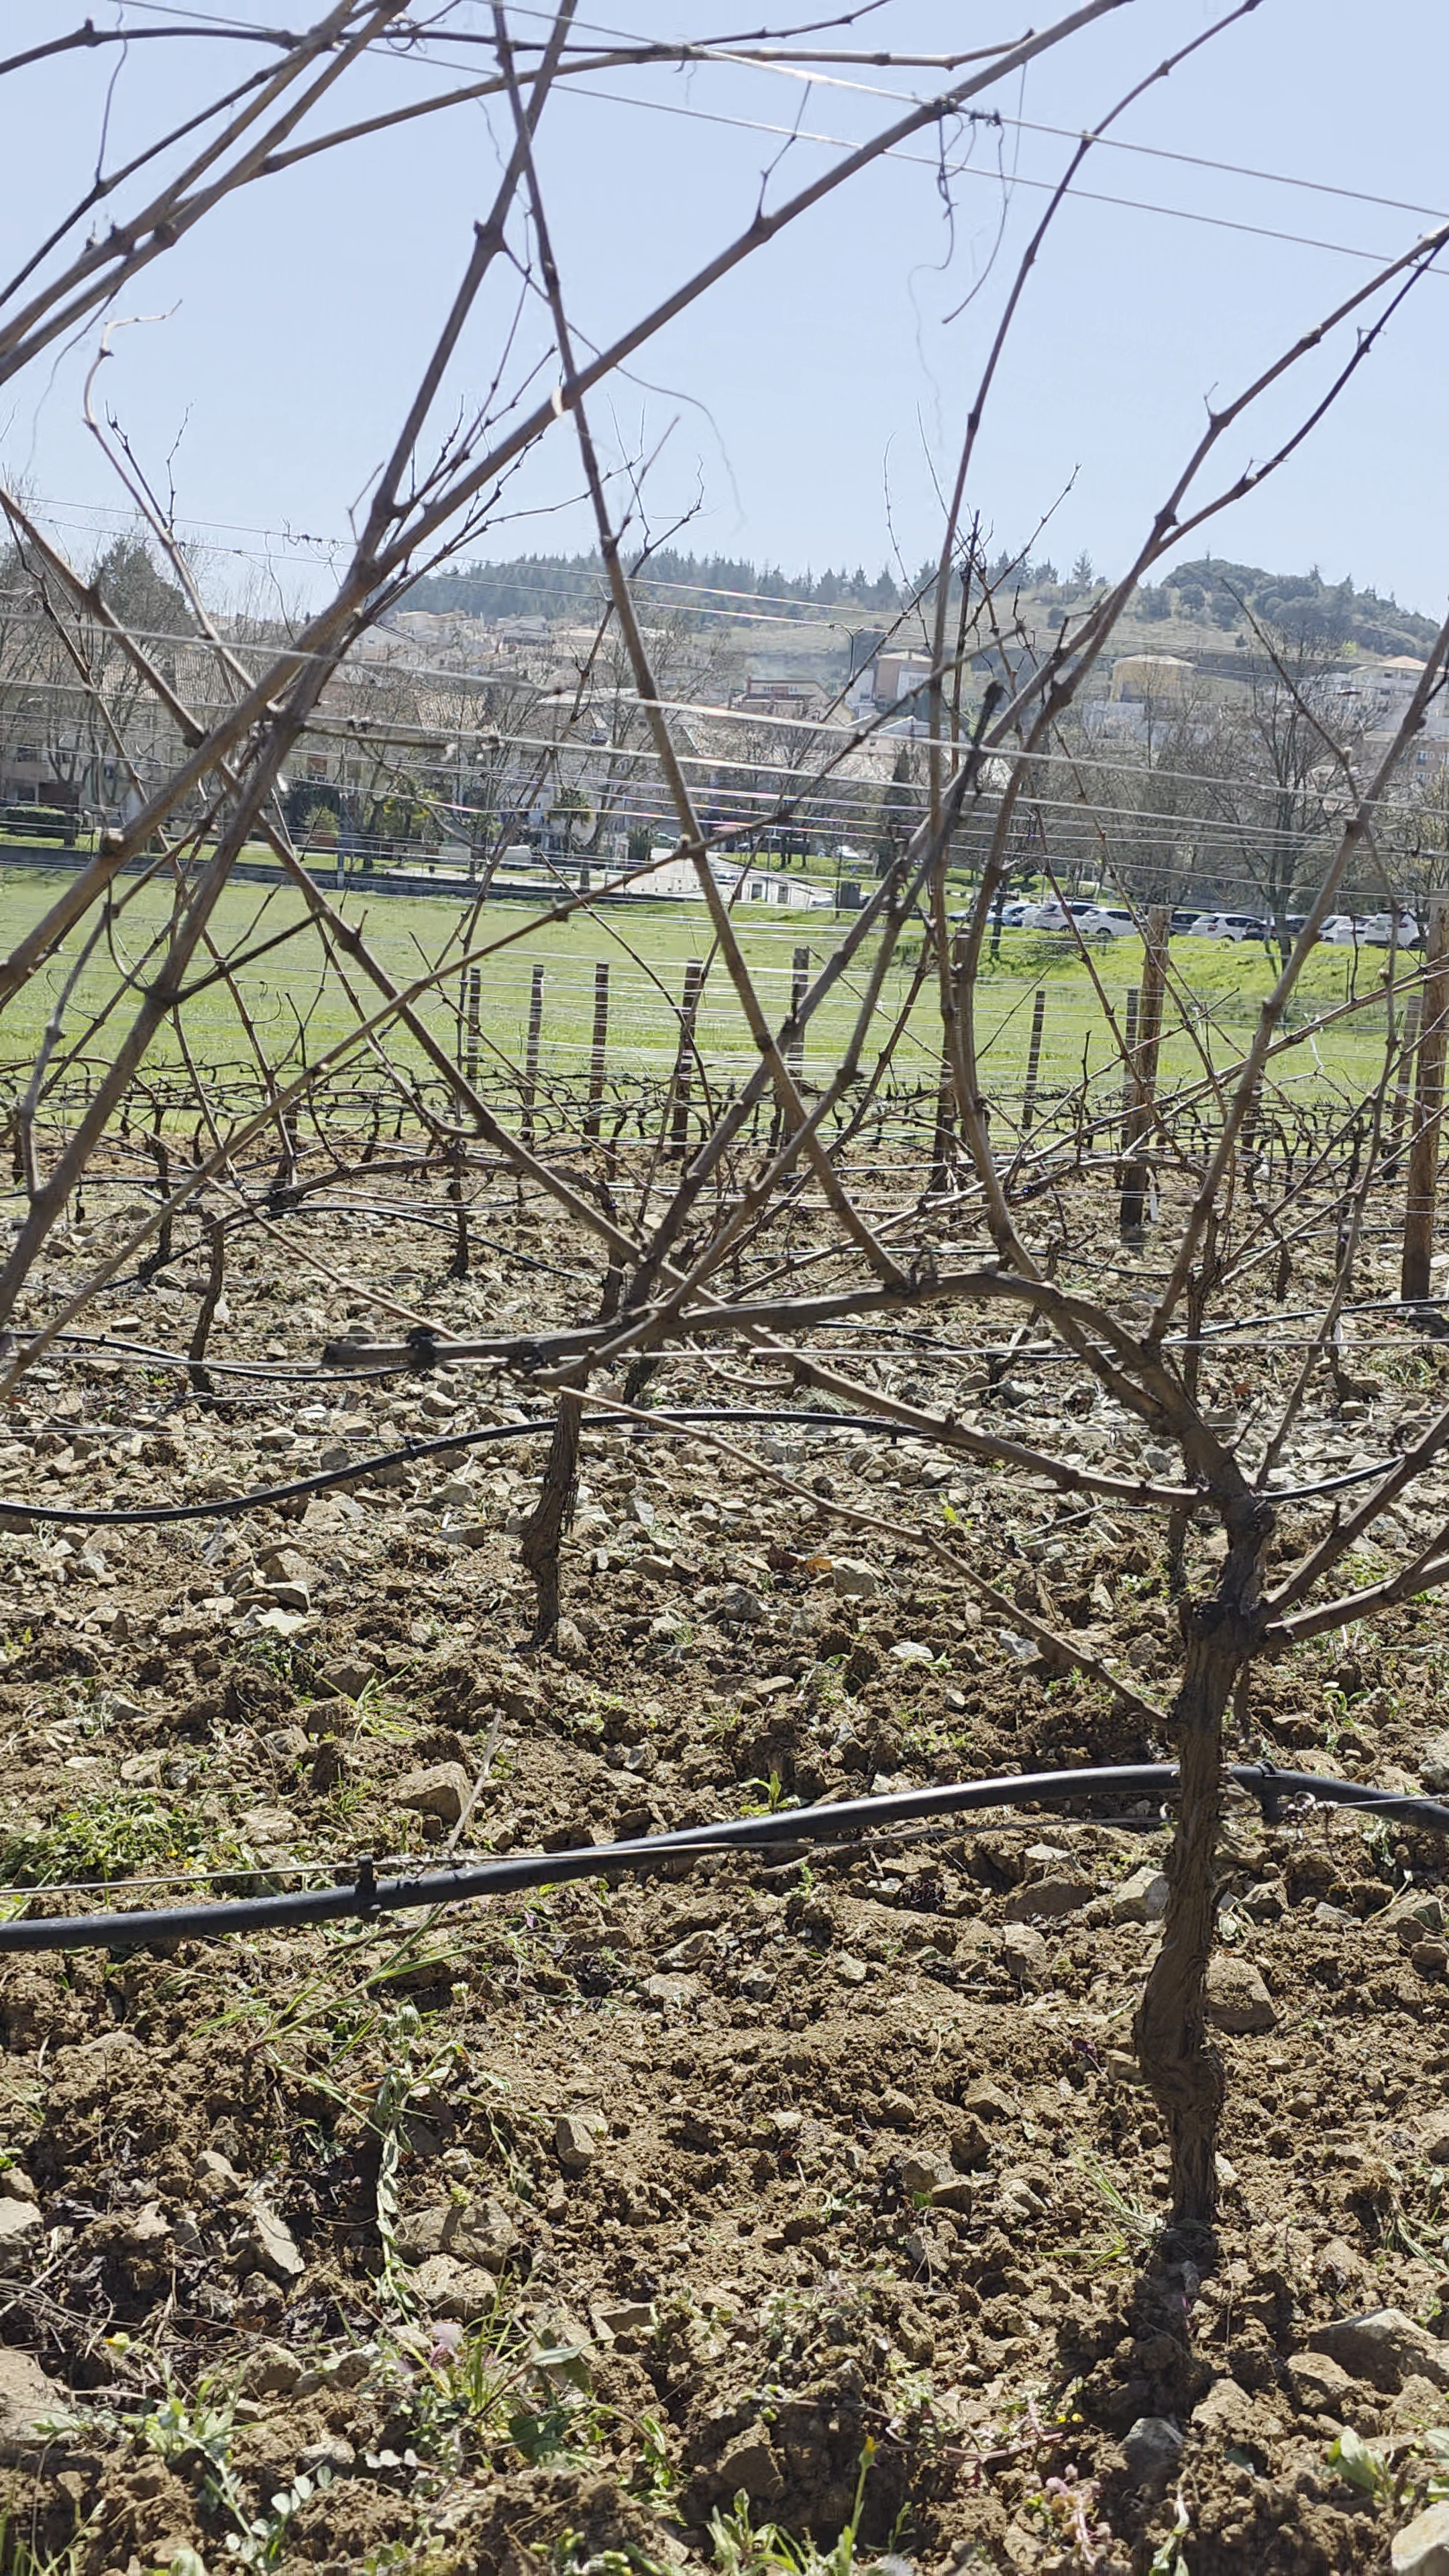
\includegraphics[width=\textwidth]{imagens/videiras_palmela.jpg}
    \caption{Imagem original (sem anotações)}
  \end{subfigure}
  \hfill
  \begin{subfigure}[b]{0.48\textwidth}
    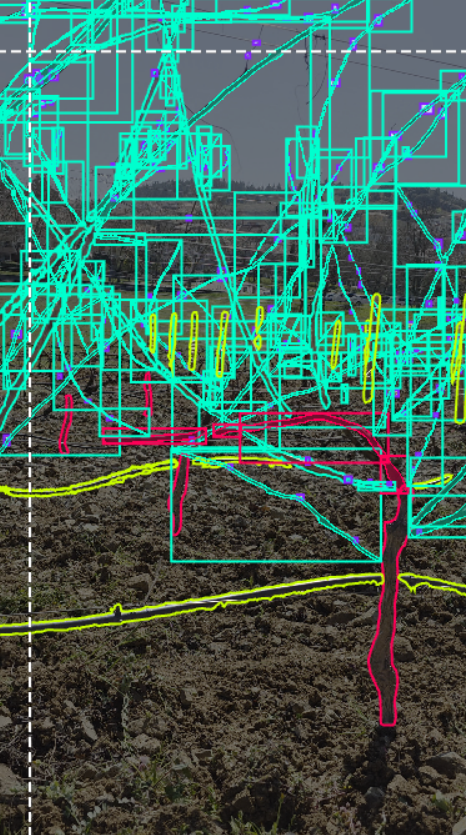
\includegraphics[width=\textwidth]{imagens/videiras_anotadas.png}
    \caption{Mesma imagem com anotações (\textgreater 300 \textit{bounding boxes})}
  \end{subfigure}
  \caption{Exemplo de imagem das vinhas de Palmela antes e após anotação manual,
           ilustrando a elevada densidade de instâncias por frame.}
  \label{fig:anotacao_exemplo}
\end{figure}

\begin{figure}[H]
  \centering
  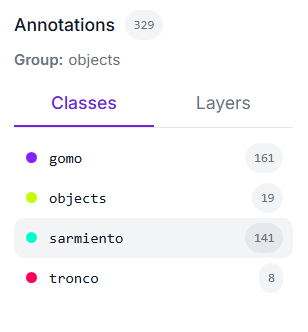
\includegraphics[width=0.75\textwidth]{imagens/Classes_videira_anotada.png}
  \caption{Distribuição do número de instâncias anotadas por classe na imagem de exemplo.}
  \label{fig:classes_contagem}
\end{figure}

\section{Arquitetura do Sistema}

\subsection{Modelo: YOLO26 Nano}

O modelo de deteção selecionado foi o \textbf{YOLO26 Nano}, a versão mais
recente da família YOLO (\textit{You Only Look Once}), desenvolvida pela
Ultralytics e documentada por Hidayatullah e
Tubagus~\cite{hidayatullah2026yolo26}. Lançado em janeiro de 2026 com o
lema \textit{"Built End-to-End. Built for the Edge"}, o YOLO26 foi
concebido para maximizar a eficiência em dispositivos de baixo custo
computacional, mantendo elevada precisão. A escolha recaiu sobre a variante
\textbf{Nano} (a mais leve da família) pelos seguintes motivos:

\begin{itemize}
  \item \textbf{Inferência sem NMS (\textit{Non-Maximum Suppression}):}
    Versões anteriores do YOLO necessitavam de uma etapa de
    pós-processamento chamada NMS, que filtrava deteções sobrepostas
    calculando a interseção sobre a união (\textit{IoU}) entre caixas.
    O YOLO26 elimina esta etapa através de inferência \textit{End-to-End
    NMS-Free}: durante o treino são utilizadas duas cabeças de deteção
    simultâneas (\textit{one-to-many} e \textit{one-to-one}); na inferência
    apenas a cabeça \textit{one-to-one} é usada, produzindo diretamente um
    conjunto limitado de deteções de alta confiança sem necessidade de
    filtragem posterior. O resultado é uma redução de 43\% na latência no
    modo CPU face ao YOLOv8.

  \item \textbf{Eliminação da DFL (\textit{Distribution Focal Loss}):}
    Versões anteriores estimavam as caixas delimitadoras como distribuições
    de probabilidade (DFL), adicionando complexidade computacional e
    dependência do NMS. O YOLO26 substitui esta abordagem por regressão
    direta de coordenadas, simplificando o \textit{pipeline} de treino e
    inferência.

  \item \textbf{SPPF com atalho residual (\textit{Spatial Pyramid Pooling
    Fast}):} O bloco SPPF, que agrega características a múltiplas escalas,
    passa a incluir uma ligação residual (\textit{shortcut}), melhorando
    o fluxo de gradiente e a estabilidade do treino.

  \item \textbf{PSABlock (\textit{Polarized Self-Attention Block}):}
    O último bloco C3k2 do \textit{neck} incorpora um mecanismo de atenção
    global (PSABlock), melhorando a modelação de contexto sem aumento
    significativo de parâmetros ou latência.

  \item \textbf{STAL (\textit{Small-Target-Aware Label Assignment}):}
    Melhoria sobre o método de atribuição de etiquetas TAL
    (\textit{Task Alignment Learning}), que ignorava objetos muito pequenos.
    O STAL garante um mínimo de quatro âncoras para objetos com dimensão
    inferior a 8$\times$8~px (numa imagem de 640$\times$640~px) — relevante
    para a deteção de gomos de pequena dimensão nas imagens de campo.

  \item \textbf{ProgLoss (\textit{Progressive Loss Balancing}):}
    Ajusta dinamicamente o peso de cada cabeça de deteção ao longo do
    treino: nas primeiras épocas, a cabeça \textit{one-to-many} recebe
    maior peso para estabilizar a aprendizagem; progressivamente, o peso
    transfere-se para a cabeça \textit{one-to-one}, alinhando o treino com
    o comportamento de inferência.

  \item \textbf{MuSGD (\textit{Muon Stochastic Gradient Descent}):}
    Otimizador híbrido que combina o SGD (\textit{Stochastic Gradient
    Descent}) clássico com atualizações estilo Muon (originalmente
    desenvolvido para treino de LLMs — \textit{Large Language Models}).
    O resultado é uma convergência mais rápida e estável, especialmente
    em datasets de dimensão reduzida.

  \item \textbf{Suporte a \textit{transfer learning}:} Os pesos
    pré-treinados no dataset COCO permitem uma inicialização favorável,
    acelerando a convergência mesmo com datasets de pequena dimensão.
\end{itemize}

A Figura~\ref{fig:yolo26_arch} apresenta o diagrama detalhado da arquitetura
do YOLO26, o primeiro diagrama publicado para este
modelo~\cite{hidayatullah2026yolo26}. A arquitetura organiza-se em três
regiões: \textbf{Backbone} (blocos C3k2 com convoluções de \textit{stride} 2
para extração de características a quatro escalas), \textbf{Neck} (SPPF com
atalho residual + C2PSA com PSABlock de atenção global + blocos de
\textit{upsample} e concatenação) e \textbf{Head} (três cabeças de deteção
para objetos pequenos, médios e grandes).

\begin{figure}[H]
  \centering
  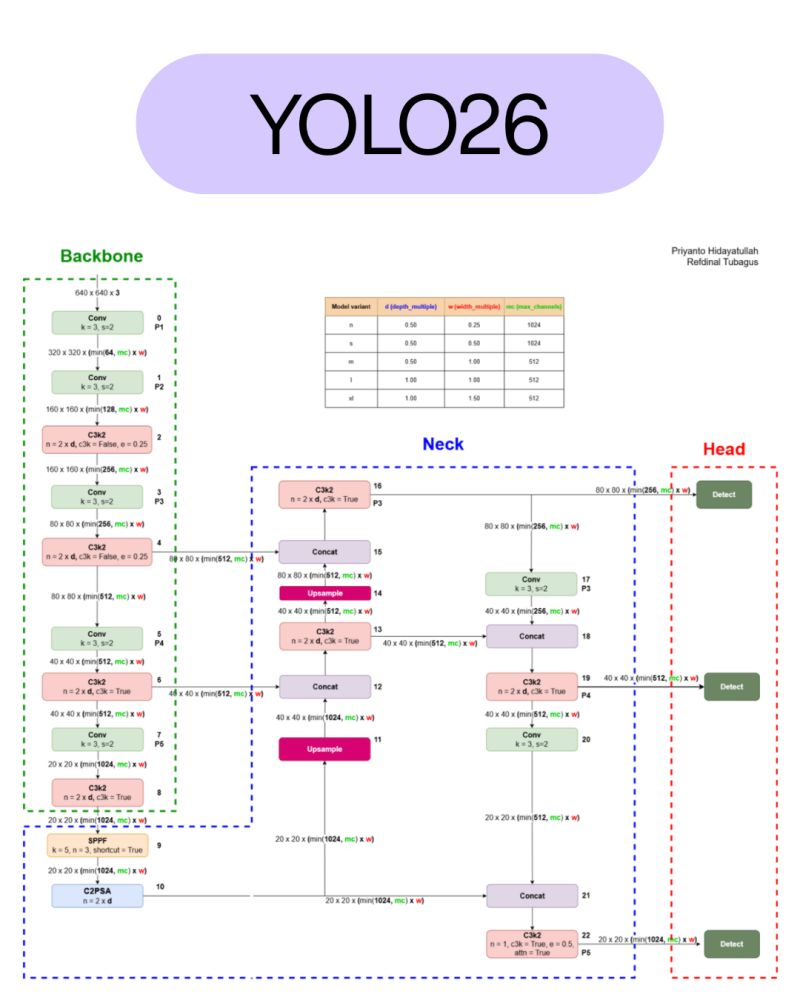
\includegraphics[width=0.92\textwidth]{imagens/YOLOV26_ARCH.jpg}
  \caption{Diagrama de arquitetura do YOLO26 Nano: Backbone (C3k2 + SPPF
           com atalho residual), Neck (C2PSA com PSABlock de atenção) e
           três cabeças de deteção (\textit{small}, \textit{medium},
           \textit{large}). Fonte:~\cite{hidayatullah2026yolo26}.}
  \label{fig:yolo26_arch}
\end{figure}

\subsection{Configuração do Dataset — \texttt{data.yaml}}

A organização do dataset segue a estrutura padrão do YOLO, com as pastas
\texttt{train/}, \texttt{valid/} e \texttt{test/}, cada uma contendo as
sub-pastas \texttt{images/} e \texttt{labels/}. O ficheiro \texttt{data.yaml}
descreve o dataset ao modelo:

\begin{lstlisting}[language=yaml, caption={Exemplo de \texttt{data.yaml} para o dataset de Palmela}]
path: /datasets/palmela_v1
train: train/images
val:   valid/images
test:  test/images

nc: 4
names:
  0: gomo
  1: sarmento
  2: tronco
  3: objeto
\end{lstlisting}

\subsection{Scripts de Download Automatizado}

Para automatizar o download de datasets do Roboflow, foi desenvolvido um
script Python que utiliza a API da plataforma:

\begin{lstlisting}[language=Python, caption={Download automático de dataset via API Roboflow}]
from roboflow import Roboflow

rf = Roboflow(api_key="SUA_API_KEY")
project = rf.workspace("nome-workspace").project("nome-projeto")
dataset  = project.version(1).download("yolov8")
\end{lstlisting}

\section{Procedimento de Treino}

O treino dos modelos foi realizado diretamente na plataforma \textbf{Roboflow},
recorrendo à funcionalidade de treino na nuvem (\textit{Roboflow Train}).
Esta abordagem dispensa a configuração de um ambiente local com GPU,
uma vez que a plataforma disponibiliza infraestrutura de computação gerida.

O processo de treino na plataforma segue os seguintes passos:

\begin{enumerate}
  \item Selecionar a versão do dataset a treinar no projeto Roboflow;
  \item Escolher o modelo base — foi utilizado o \textbf{YOLO26 Nano} com pesos
    pré-treinados no COCO;
  \item Definir o número de épocas e iniciar o treino;
  \item Acompanhar as métricas de desempenho (mAP, Precisão, Recall) em
    tempo real no painel da plataforma;
  \item Descarregar os pesos do modelo treinado (\texttt{best.pt}) após
    conclusão.
\end{enumerate}

\begin{table}[H]
  \centering
  \caption{Configuração de treino no Roboflow Train}
  \label{tab:hyperparams}
  \begin{tabular}{ll}
    \toprule
    \textbf{Parâmetro}       & \textbf{Valor} \\
    \midrule
    Plataforma de treino     & Roboflow Train (nuvem) \\
    Modelo base              & YOLO26 Nano (COCO) \\
    Épocas (\texttt{epochs}) & 100 \\
    Tamanho de imagem        & 640 \\
    Divisão treino/val/teste & 70\% / 20\% / 10\% \\
    Pesos exportados         & \texttt{best.pt} (formato PyTorch) \\
    \bottomrule
  \end{tabular}
\end{table}

%==========================================================================
% CAPÍTULO 4 — DESENVOLVIMENTO
%==========================================================================
\chapter{Desenvolvimento}
\label{chap:desenvolvimento}

% ------------------------------------------------------------------
% Nota sobre Data Augmentation
% ------------------------------------------------------------------
\section*{Nota sobre Contagem de Imagens}
\addcontentsline{toc}{section}{Nota sobre Contagem de Imagens}

Durante o treino na plataforma Roboflow Train, a plataforma aplica
automaticamente técnicas de \textit{data augmentation} (rotações,
espelhos, variações de brilho e contraste, entre outras) sobre as
imagens anotadas. Os valores de contagem de imagens reportados no
painel do Roboflow referem-se sempre ao total \textbf{após
augmentation}, e não ao número de imagens base originalmente anotadas.

A Tabela~\ref{tab:datasets_aug} resume a composição de cada versão
do dataset, distinguindo as contagens base das contagens pós-augmentation.

\begin{table}[H]
  \centering
  \caption{Composição dos datasets por modelo (imagens base vs.\
           após \textit{data augmentation})}
  \label{tab:datasets_aug}
  \begin{tabularx}{\textwidth}{l c c c X}
    \toprule
    \textbf{Modelo} & \textbf{Base SVY-2} & \textbf{Base Palmela}
                    & \textbf{Base total} & \textbf{Após augmentation (Roboflow)} \\
    \midrule
    Modelo 1 & 300 & 0   & 300  & $\approx$775 \\
    Modelo 2 & 300 & 100 & 400  & 772 \\
    Modelo 3 & 300 & 100+ & 400+ & 938 \\
    \bottomrule
  \end{tabularx}
\end{table}

% ------------------------------------------------------------------
\section{Modelo 1 — \textit{Segmentation-Vineyard-2} (fase de validação técnica)}
% ------------------------------------------------------------------

\subsection{Caracterização do Dataset}

O primeiro modelo foi desenvolvido com base no dataset público
\textbf{Segmentation-Vineyard-2}~\cite{vinya2024segvineyard}, disponível na
plataforma Roboflow Universe e de origem espanhola. Este dataset continha
originalmente apenas anotações de \texttt{sarmento} e \texttt{tronco} —
não incluía qualquer anotação de gomos.

A contribuição deste estágio consistiu em anotar manualmente os
gomos em cada uma das 300 imagens do dataset, acrescentando a classe
\texttt{gomo} ao conjunto de etiquetas existente. O Modelo~1 passou assim
a ter três classes: \texttt{gomo}, \texttt{sarmento} e \texttt{tronco}.
O dataset foi dividido na plataforma Roboflow nas proporções
70\% treino / 20\% validação / 10\% teste. Após a aplicação de
\textit{data augmentation} pelo Roboflow, o conjunto de treino
atingiu aproximadamente 775 imagens.

O processo de desenvolvimento do Modelo~1 serviu como etapa de validação
da \textit{pipeline} técnica e permitiu confirmar a viabilidade do fluxo
completo de anotação, treino e inferência antes de introduzir as imagens
de Palmela, de maior complexidade.

\subsection{Refinamento das Etiquetas}

Após uma inspeção visual inicial do \textbf{Segmentation-Vineyard-2}, foram identificadas
algumas inconsistências nas anotações de \texttt{sarmento} e \texttt{tronco}
— \textit{bounding boxes} excessivamente largas ou com sobreposição não
intencional. Procedeu-se ao refinamento manual de parte dessas anotações,
em simultâneo com a adição das anotações de \texttt{gomo}.

\subsection{Observações Qualitativas}

A inferência sobre imagens do conjunto de teste revelou que o modelo
identifica corretamente os sarmentos com elevada confiança (até 97\%)
e os troncos com boa confiança (acima de 83\%). As métricas formais
deste modelo foram obtidas apenas na versão do Roboflow correspondente
ao Modelo~2 (que utilizou o mesmo dataset base acrescido das imagens de
Palmela), dado que ambas as versões foram treinadas numa única sessão
sequencial na plataforma.

% ------------------------------------------------------------------
\section{Modelo 2 — SVY-2 + Palmela (400 imagens base)}
\label{sec:modelo2}
% ------------------------------------------------------------------

\subsection{Justificação e Contexto}

O desenvolvimento do segundo modelo representa o núcleo do trabalho prático
deste estágio. A motivação para a criação de um novo dataset, em vez de
reutilizar integralmente o dataset espanhol, reside na diferença substancial
entre as condições das imagens disponíveis publicamente e as condições reais
de operação de um robô de poda nas vinhas portuguesas.

As imagens do \textbf{Segmentation-Vineyard-2} foram, na sua maioria, captadas em condições
controladas ou com planos de fundo limpos. Em contrapartida, um robô real
que percorra as vinhas de Palmela capturará cenas com:

\begin{itemize}
  \item Múltiplas videiras visíveis em simultâneo (primeiro e segundo planos);
  \item Arames de suporte, postes e outros elementos de infraestrutura;
  \item Reflexos de luz solar e variações abruptas de contraste;
  \item Sarmentos de diferentes espessuras e comprimentos que se cruzam
    e sobrepõem no campo visual.
\end{itemize}

É precisamente esta realidade que o Modelo~2 pretende capturar.

\subsection{Processo de Captação de Vídeo}

Os vídeos utilizados para construir o dataset de Palmela foram captados
durante uma visita às vinhas da região, realizada em março de 2026. A
captação foi efetuada com câmera de smartphone em modo vídeo, percorrendo
as fileiras de videiras a pé, de forma a simular o deslocamento de um
robô agrícola.

Para cobrir diferentes perspetivas e condições de iluminação, foram
realizadas passagens ao longo de várias filas em diferentes horas do dia.
A taxa de captura foi configurada em \textbf{2 frames por segundo} no
Roboflow, o que corresponde a uma amostragem suficiente para capturar a
diversidade visual sem criar um número excessivo de frames redundantes.

\subsection{Importação e Extração de Frames no Roboflow}

Os ficheiros de vídeo (formato \texttt{.mp4}) foram importados diretamente
para o projeto no Roboflow. A plataforma realiza automaticamente a extração
dos frames à taxa configurada e apresenta-os sequencialmente para anotação.
Esta funcionalidade reduziu significativamente o tempo de pré-processamento
manual dos dados.

\subsection{Evolução da Estratégia de Anotação}

Ao longo das sessões de anotação do dataset de Palmela, a estratégia foi
sendo refinada com base nas dificuldades encontradas. A decisão de incluir
as classes \texttt{tronco} e \texttt{objeto} surgiu após as primeiras experiências
de treino revelarem que o modelo confundia estes elementos com sarmentos e
gomos.

A inclusão dos sarmentos como classe própria — e não apenas como
contexto — foi igualmente determinante. Ao delimitar os sarmentos, o modelo
adquire um guia estrutural que facilita a localização dos gomos, que crescem
ao longo dos sarmentos em posições relativamente regulares.

\subsection{Dificuldades Específicas e Decisões Tomadas}

\paragraph{Densidade de instâncias por imagem.}
Cada imagem das vinhas de Palmela pode conter dezenas de gomos visíveis.
A política de anotação adoptada foi a de marcar o máximo de gomos
identificáveis em cada imagem. Esta decisão baseia-se numa característica
biológica favorável: os gomos crescem em posições regulares e previsíveis ao
longo dos sarmentos, pelo que os seus locais de inserção são reconhecíveis
mesmo a distância ou em condições de visibilidade parcial. Omitir gomos
identificáveis introduziria falsos negativos sistemáticos no treino,
prejudicando a capacidade de \textit{recall} do modelo.

\paragraph{Ambiguidade de fronteiras entre classes.}
Em certas imagens, a distinção entre um sarmento em primeiro plano e um
tronco em segundo plano é subjetiva. Foi adotada a regra de que a classe é
determinada pela posição relativa ao plano focal principal: o elemento mais
próximo da câmera é classificado pelo seu tipo real.

\paragraph{Gomos muito pequenos.}
Em imagens captadas a maior distância, os gomos aparecem com dimensões
inferiores a 15$\times$15~px. Estes casos foram anotados quando identificáveis,
mas reconhece-se que o modelo terá maior dificuldade em detetá-los.

\subsection{Estado da Anotação e Métricas}

Até à data de elaboração deste relatório, foram anotadas aproximadamente
100 imagens provenientes das vinhas de Palmela, que foram
combinadas com as 300 imagens do Segmentation-Vineyard-2 para compor o
dataset do Modelo~2 (400 imagens base no total). Após a aplicação de
\textit{data augmentation} pelo Roboflow, o conjunto de treino atingiu
772 imagens, divididas nas proporções 70\% treino / 20\% validação /
10\% teste.

A Tabela~\ref{tab:resultados_m2_dev} apresenta as métricas obtidas no
conjunto de validação.

\begin{table}[H]
  \centering
  \caption{Métricas do Modelo 2 no conjunto de validação (Roboflow Train)}
  \label{tab:resultados_m2_dev}
  \begin{tabular}{lc}
    \toprule
    \textbf{Métrica}   & \textbf{Valor} \\
    \midrule
    mAP@50             & 48,8\% \\
    Precisão           & 54,3\% \\
    Recall             & 52,7\% \\
    F1-Score           & 53,5\% \\
    \bottomrule
  \end{tabular}
\end{table}

Os resultados são moderados mas coerentes com a natureza do Modelo~2:
dataset de domínio misto (espanhol + português), quatro classes com
densidades de instâncias muito distintas, e uma classe (\texttt{gomo})
completamente nova relativamente ao dataset base. A precisão de 54,3\%
e o recall de 52,7\% equilibrados indicam que o modelo distribui as
dificuldades de forma homogénea, sem enviesamento sistemático.

O dataset encontra-se versionado no Roboflow, permitindo reprodutibilidade
dos treinos e rastreabilidade das alterações de anotação.

% ------------------------------------------------------------------
\section{Modelo 3 — Dataset Expandido (400+ imagens base, 938 augmentadas)}
\label{sec:modelo3}
% ------------------------------------------------------------------

\subsection{Contexto e Motivação}

Com base nos resultados do Modelo~2 e na análise qualitativa das
inferências, foi construída uma terceira versão do dataset com imagens
de Palmela adicionais. O objetivo foi avaliar se o aumento do volume de
dados resultaria numa melhoria das métricas, em particular no Recall da
classe \texttt{gomo}.

\subsection{Composição do Dataset e Resultados}

O dataset do Modelo~3 foi gerado em 17 de junho de 2026, com um total de
938 imagens após augmentation. A Tabela~\ref{tab:resultados_m3_dev}
resume as métricas obtidas no conjunto de validação.

\begin{table}[H]
  \centering
  \caption{Métricas do Modelo 3 no conjunto de validação (Roboflow Train)}
  \label{tab:resultados_m3_dev}
  \begin{tabular}{lc}
    \toprule
    \textbf{Métrica}   & \textbf{Valor} \\
    \midrule
    mAP@50             & 43,7\% \\
    Precisão           & 57,3\% \\
    Recall             & 40,5\% \\
    F1-Score           & 47,4\% \\
    \bottomrule
  \end{tabular}
\end{table}

A Figura~\ref{fig:resultado_m3} mostra uma inferência do Modelo~3 sobre
uma imagem das vinhas de Palmela, com \textit{confidence threshold} de 16\%.

\begin{figure}[H]
  \centering
  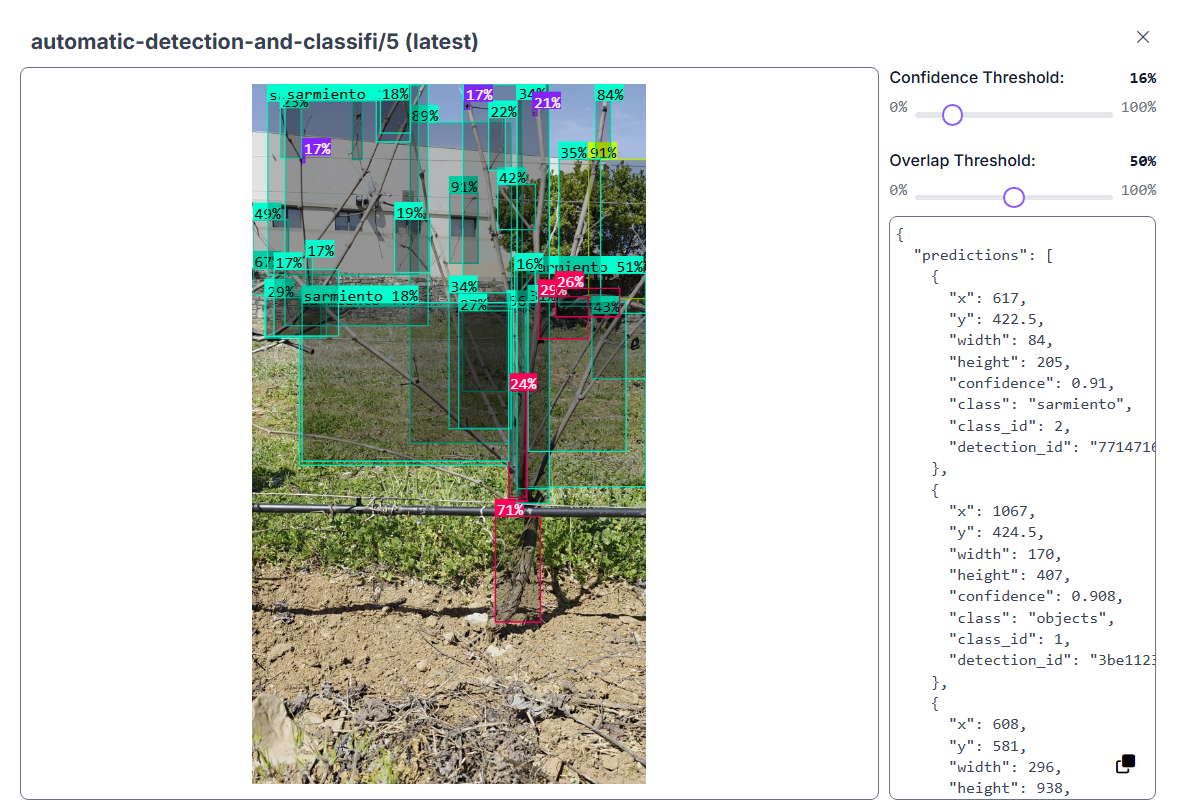
\includegraphics[width=0.85\textwidth]{imagens/resultado_v3.png}
  \caption{Inferência do Modelo~3 sobre imagem das vinhas de Palmela
           (\textit{threshold} = 16\%). Sarmentos (ciano), gomos (roxo),
           objetos (vermelho). Os sarmentos atingem confiança até 91\%;
           os gomos surgem apenas com confiança de 16--26\%, indicando
           que a classe está a ser aprendida mas requer mais dados.}
  \label{fig:resultado_m3}
\end{figure}

\subsection{Análise dos Resultados do Modelo 3}

A comparação entre o Modelo~2 (mAP@50 = 48,8\%) e o Modelo~3
(mAP@50 = 43,7\%) revela uma descida ligeira nas métricas globais, que
se explica pelo aumento da complexidade do dataset — mais imagens de
Palmela com maior densidade de instâncias e mais variação visual. Não
obstante, a Precisão subiu de 54,3\% para 57,3\%, o que indica menos
falsos positivos. O Recall de 40,5\% reflete a dificuldade em detetar
gomos com confiança suficiente para ultrapassar o limiar de 50\%.

A análise da inferência (Figura~\ref{fig:resultado_m3}) revela que:
\begin{itemize}
  \item Os sarmentos são detetados com elevada confiança (até 91\%);
  \item Um objeto (estaca/poste) é detetado corretamente com 71\% de confiança;
  \item Os gomos surgem com confiança de 16--26\%, indicando que o modelo
    está a aprender a classe, mas o volume de dados ainda é insuficiente
    para calibrar a confiança neste nível.
\end{itemize}

Este comportamento é esperado para uma classe de pequena dimensão com
elevada variabilidade intra-classe e volume de dados limitado.

% ------------------------------------------------------------------
\section{Considerações sobre a Complexidade do Problema}
% ------------------------------------------------------------------

A experiência acumulada durante o estágio permite afirmar que a tarefa de
deteção de gomos em cenas reais de vinha, com a complexidade visual observada
nas imagens de Palmela, é um problema que excede o que pode ser
resolvido satisfatoriamente num único semestre de trabalho. As razões são
múltiplas:

\begin{enumerate}
  \item Volume de dados: modelos de deteção de objetos em cenas
    complexas tipicamente requerem milhares de imagens anotadas por classe.
    Com 100 imagens de Palmela (400+ no total com as espanholas), o modelo
    está limitado na sua capacidade de generalização.

  \item Complexidade de anotação: a anotação de imagens com grande
    densidade de instâncias é demorada e exige consistência. A taxa de
    anotação estimada é de 15--25 imagens por hora para imagens de alta
    densidade.

  \item Variabilidade do domínio: as condições de iluminação,
    fenologia e morfologia variam significativamente entre épocas do ano,
    o que implica a necessidade de múltiplas rondas de captura.

  \item Otimização do modelo: a escolha dos hiperparâmetros e das
    técnicas de \textit{data augmentation} adequadas ao domínio específico
    requer múltiplas iterações de treino e avaliação.
\end{enumerate}

Não obstante, o trabalho desenvolvido até ao momento estabelece uma base
metodológica sólida e fornece uma avaliação realista dos desafios envolvidos,
constituindo um ponto de partida valioso para projetos de continuação.

%==========================================================================
% CAPÍTULO 5 — RESULTADOS PARCIAIS
%==========================================================================
\chapter{Resultados Parciais}
\label{chap:resultados}

\section{Nota Preliminar}

O presente capítulo reporta os resultados obtidos até à data de elaboração
deste relatório. Foram treinados três modelos progressivos sobre datasets
de complexidade crescente, todos utilizando a plataforma Roboflow Train
com o modelo base YOLO26 Nano. As contagens de imagens indicadas
referem-se sempre ao total após a aplicação de \textit{data augmentation}
pelo Roboflow.

\section{Métricas de Avaliação}

Para avaliar o desempenho dos modelos, são utilizadas as seguintes métricas
padrão na literatura de deteção de objetos:

\begin{description}
  \item[Precisão (P):] Fração das deteções positivas que são corretas.
    \[
      P = \frac{TP}{TP + FP}
    \]

  \item[Recall (R):] Fração dos objetos reais que foram detetados.
    \[
      R = \frac{TP}{TP + FN}
    \]

  \item[F1-Score:] Média harmónica entre Precisão e Recall.
    \[
      F1 = 2 \cdot \frac{P \cdot R}{P + R}
    \]

  \item[mAP@50:] \textit{Mean Average Precision} com limiar de IoU de 0,50.
    Métrica principal utilizada para comparação de modelos na literatura.

  \item[mAP@50-95:] Média do mAP calculado para limiares de IoU de 0,50
    a 0,95 (em passos de 0,05). Métrica mais exigente, adotada no COCO
    \textit{benchmark}.
\end{description}

\noindent onde $TP$ = Verdadeiros Positivos, $FP$ = Falsos Positivos,
$FN$ = Falsos Negativos.

% ------------------------------------------------------------------
\section{Resultados do Modelo 1 — \textit{Segmentation-Vineyard-2}}
% ------------------------------------------------------------------

O Modelo~1 foi treinado exclusivamente sobre as 300 imagens do
\textit{Segmentation-Vineyard-2} com as anotações de \textit{gomo}
adicionadas, resultando em aproximadamente 775 imagens após augmentation.
Este modelo serviu principalmente para validar a \textit{pipeline} técnica.
A inferência visual sobre imagens do conjunto de teste revelou que o modelo
identifica corretamente os sarmentos com elevada confiança (até 97\%) e os
troncos com boa confiança (acima de 83\%), validando a capacidade do
YOLO26 Nano de aprender a estrutura visual das videiras mesmo com datasets
de dimensão reduzida.

% ------------------------------------------------------------------
\section{Resultados do Modelo 2 — SVY-2 + Palmela}
% ------------------------------------------------------------------

A Tabela~\ref{tab:resultados_m2} apresenta as métricas obtidas pelo Modelo~2
no conjunto de validação, após treino sobre 772 imagens (augmentation de
400 imagens base: 300 do \textit{Segmentation-Vineyard-2} + 100 de Palmela).

\begin{table}[H]
  \centering
  \caption{Resultados do Modelo 2 (validação) — SVY-2 + Palmela, 772 imagens}
  \label{tab:resultados_m2}
  \begin{tabular}{lcccc}
    \toprule
    \textbf{Escopo}     & \textbf{P} & \textbf{R} & \textbf{F1} & \textbf{mAP@50} \\
    \midrule
    Todas as classes    & 54,3\%     & 52,7\%     & 53,5\%      & 48,8\%          \\
    \bottomrule
  \end{tabular}
\end{table}

\noindent\textit{Nota: O Roboflow Train, no plano gratuito, reporta apenas
métricas globais no painel principal. Os valores por classe estão disponíveis
nas ferramentas de avaliação avançada (plano pago).}

Um mAP@50 de 48,8\% é um resultado moderado mas coerente com as
condições do Modelo~2: dataset de domínio misto (espanhol + português),
quatro classes com densidades de instâncias muito distintas, e uma classe
(\textit{gomo}) completamente nova relativamente ao dataset base. A
precisão (54,3\%) e o recall (52,7\%) equilibrados indicam que o modelo
não está sistematicamente enviesado.

% ------------------------------------------------------------------
\section{Resultados do Modelo 3 — Dataset Expandido}
% ------------------------------------------------------------------

A Tabela~\ref{tab:resultados_m3} apresenta as métricas obtidas pelo Modelo~3,
treinado sobre 938 imagens (geradas por augmentation a partir das imagens
base disponíveis até 17 de junho de 2026).

\begin{table}[H]
  \centering
  \caption{Resultados do Modelo 3 (validação) — 938 imagens}
  \label{tab:resultados_m3}
  \begin{tabular}{lcccc}
    \toprule
    \textbf{Escopo}     & \textbf{P} & \textbf{R} & \textbf{F1} & \textbf{mAP@50} \\
    \midrule
    Todas as classes    & 57,3\%     & 40,5\%     & 47,4\%      & 43,7\%          \\
    \bottomrule
  \end{tabular}
\end{table}

A Figura~\ref{fig:resultado_m3_res} mostra uma inferência do Modelo~3 sobre
uma imagem das vinhas de Palmela, com \textit{confidence threshold} de 16\%.

\begin{figure}[H]
  \centering
  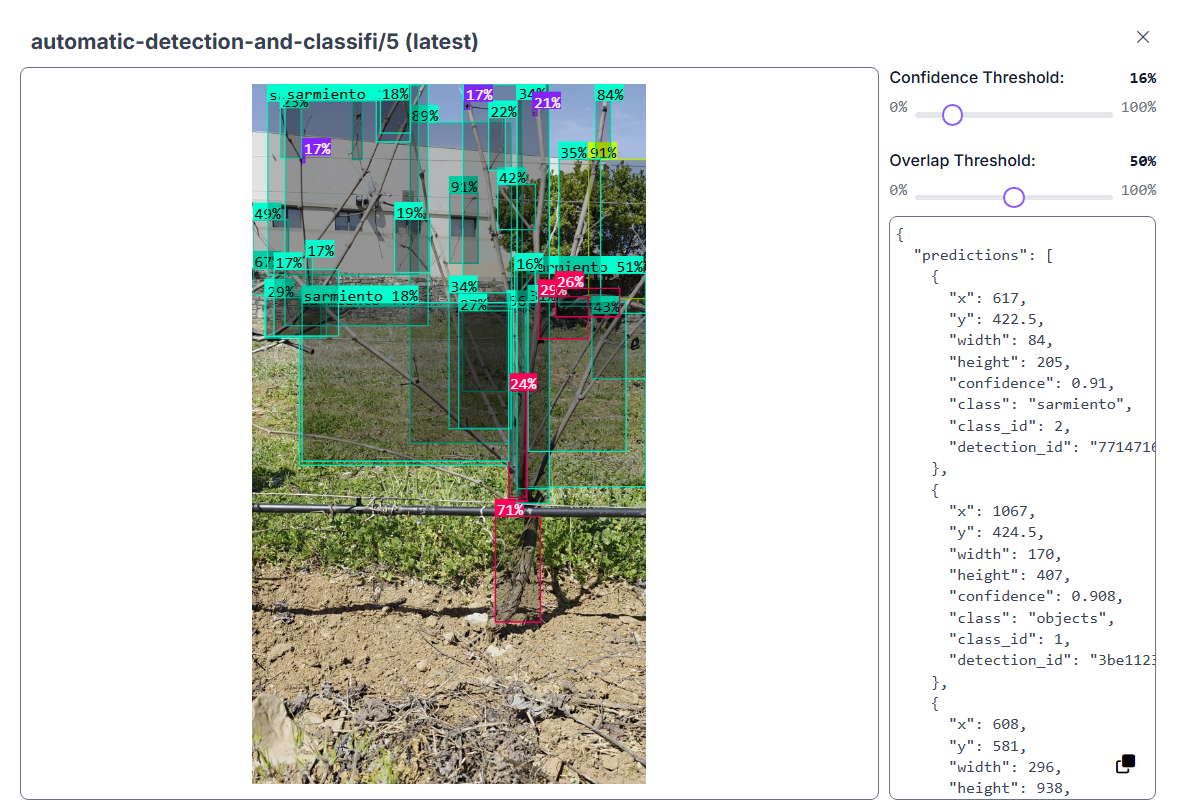
\includegraphics[width=0.80\textwidth]{imagens/resultado_v3.png}
  \caption{Inferência do Modelo~3 (threshold = 16\%). Os sarmentos (ciano)
           são detetados com confiança até 91\%; os gomos (roxo) surgem com
           confiança de 16--26\%; um obstáculo/poste é detetado a vermelho
           com 71\%.}
  \label{fig:resultado_m3_res}
\end{figure}

% ------------------------------------------------------------------
\section{Análise das Dificuldades Observadas}
% ------------------------------------------------------------------

A análise das inferências do Modelo~3 permite identificar três padrões
recorrentes de erro:

\begin{description}
  \item[Gomos com confiança insuficiente:] O modelo detecta a presença de
    gomos, mas a confiança atribuída (16--26\%) fica abaixo do limiar
    convencional de 50\%. Este padrão indica que a classe está a ser
    aprendida, mas o volume de dados de treino é ainda insuficiente para
    calibrar adequadamente a confiança.

  \item[Sarmentos de fundo confundidos com sarmentos de frente:]
    Em imagens com múltiplas videiras, sarmentos de segundo plano são
    por vezes detetados com alta confiança em detrimento dos de primeiro
    plano, pois têm maior contraste com o fundo.

  \item[Ausência de deteção de tronco em imagens de baixo contraste:]
    Em imagens com terreno de cor similar ao tronco, este não é detetado,
    apesar de estar visível.
\end{description}

% ------------------------------------------------------------------
\section{Comparação entre os Três Modelos}
% ------------------------------------------------------------------

A Tabela~\ref{tab:comparacao_modelos} resume as diferenças fundamentais
entre as três abordagens desenvolvidas neste estágio.

\begin{table}[H]
  \centering
  \caption{Comparação entre os três modelos desenvolvidos}
  \label{tab:comparacao_modelos}
  \begin{tabularx}{\textwidth}{l X X X}
    \toprule
    \textbf{Aspeto}          & \textbf{Modelo 1} & \textbf{Modelo 2} & \textbf{Modelo 3} \\
    \midrule
    Origem dos dados         & \textit{Segmentation-Vineyard-2} & SVY-2 + Palmela & SVY-2 + Palmela \\
    Imagens base             & $\approx$300      & $\approx$400      & $\approx$400+    \\
    Imagens (aug.)           & $\approx$775      & 772               & 938              \\
    N.º de classes           & 3                 & 4                 & 4                \\
    Complexidade das imagens & Moderada          & Alta              & Alta             \\
    Aplicabilidade real      & Limitada          & Alta              & Alta             \\
    mAP@50                   & ---               & 48,8\%            & 43,7\%           \\
    Precisão                 & ---               & 54,3\%            & 57,3\%           \\
    Recall                   & ---               & 52,7\%            & 40,5\%           \\
    F1                       & ---               & 53,5\%            & 47,4\%           \\
    Estado                   & Concluído         & Concluído         & Ativo            \\
    \bottomrule
  \end{tabularx}
\end{table}

A transição do Modelo~2 para o Modelo~3 evidencia um padrão coerente com
o aumento da dificuldade do dataset: o mAP@50 desce de 48,8\% para 43,7\%,
mas a Precisão sobe de 54,3\% para 57,3\% (menos falsos positivos). A
queda no Recall de 52,7\% para 40,5\% reflete principalmente a dificuldade
de detetar gomos com confiança suficiente nas novas imagens de Palmela,
mais complexas e variadas.

%==========================================================================
% CAPÍTULO 6 — CONCLUSÃO E TRABALHOS FUTUROS
%==========================================================================
\chapter{Conclusão e Trabalhos Futuros}
\label{chap:conclusao}

\section{Conclusão}

O presente estágio teve como objetivo investigar a viabilidade de um sistema
de \textbf{deteção automática de gomos em videiras} utilizando técnicas de
visão computacional e \textit{deep learning}, com vista à sua integração num
futuro sistema robótico de poda mecanizada.

Ao longo do período de estágio foram desenvolvidas duas abordagens
complementares. O \textbf{Modelo~1}, baseado num dataset espanhol de domínio
público, permitiu validar a \textit{pipeline} técnica e demonstrar que o
    YOLO26 Nano é capaz de detetar gomos em condições de imagem moderadamente
controladas. O \textbf{Modelo~2}, construído a partir de vídeos captados nas
vinhas de Palmela, representa um esforço mais ambicioso e realista, visando
treinar um modelo robusto em condições próximas de uma operação robótica real.

Os principais resultados e contribuições do estágio são:

\begin{itemize}
  \item Construção de uma metodologia de aquisição e anotação de imagens
    adaptada à complexidade do ambiente vitícola português;

  \item Desenvolvimento de um dataset original com aproximadamente
    \textbf{400 imagens anotadas} de vinhas da região de Palmela, com
    quatro classes:     \textit{gomo}, \textit{sarmento}, \textit{tronco} e
    \textit{objeto};

  \item Identificação e documentação dos principais \textbf{desafios
    técnicos} associados à deteção de gomos em cenas reais: oclusões, fundo
    denso, variações de iluminação e alta densidade de instâncias;

  \item Avaliação da adequação do \textbf{YOLO26 Nano} para esta tarefa,
    com identificação dos seus pontos fortes (eficiência computacional,
    facilidade de integração) e limitações (sensibilidade ao volume e
    qualidade dos dados de treino);

  \item Prova de conceito de que, com um dataset suficientemente grande e
    diverso, um modelo de deteção de objetos pode localizar gomos e
    sarmentos em imagens de campo com complexidade real.
\end{itemize}

É importante reconhecer que a obtenção de um modelo plenamente funcional e
robusto para uso em sistemas robóticos reais \textbf{excede o âmbito de um
único semestre de estágio}. A complexidade visual das imagens de Palmela,
combinada com a necessidade de volumes de dados elevados, exige um esforço
continuado. Contudo, as bases estabelecidas neste trabalho são um ponto de
partida sólido e documentado para projetos de continuação.

\section{Trabalhos Futuros}

Com base na experiência adquirida e nas limitações identificadas, propõem-se
as seguintes linhas de trabalho futuro:

\subsection{Expansão e Diversificação do Dataset}

\begin{itemize}
  \item Aumentar o dataset de Palmela para um mínimo de \textbf{1000--2000
    imagens anotadas}, cobrindo diferentes épocas do ano (pré-poda, pós-
    poda, início do abrolhamento) e diferentes condições meteorológicas.

  \item Incorporar imagens de outras regiões vitivinícolas portuguesas e
    de diferentes cultivares, para aumentar a diversidade do modelo.

  \item Explorar a \textbf{anotação semi-automática}: usar um modelo
    preliminar para gerar sugestões de anotação que sejam depois revistas
    manualmente, reduzindo o esforço por imagem.
\end{itemize}

\subsection{Arquiteturas de Modelo Mais Avançadas}

\begin{itemize}
  \item Avaliar variantes maiores do YOLO26 (Small, Medium) ou modelos da
    geração seguinte (RT-DETR, YOLO-NAS) para determinar se o ganho
    em desempenho justifica o custo computacional adicional.

  \item Explorar a \textbf{segmentação de instâncias} (YOLO26-Seg) em vez
    de apenas \textit{bounding boxes}, o que poderia fornecer informação
    mais precisa sobre a geometria dos sarmentos, útil para o cálculo do
    ponto de corte.

  \item Investigar modelos baseados em \textit{transformers} para visão
    (DETR, Grounding DINO) que possam lidar melhor com oclusões severas.
\end{itemize}

\subsection{Integração com Informação de Profundidade}

A adição de uma câmera de profundidade (RGB-D) ao sistema permitiria:

\begin{itemize}
  \item Separar objetos em primeiro e segundo plano com base na distância,
    reduzindo a confusão entre sarmentos de diferentes planos;

  \item Calcular as coordenadas 3D dos gomos para guiar o braço robótico
    ao ponto de corte preciso.
\end{itemize}

\subsection{Validação em Ambiente Real}

\begin{itemize}
  \item Integrar o modelo desenvolvido num protótipo robótico e realizar
    testes \textit{in situ} nas vinhas de Palmela;

  \item Definir métricas de desempenho operacional (taxa de gomos
    corretamente identificados por metro linear de vinha, tempo de
    processamento por frame).
\end{itemize}

\subsection{Técnicas de \textit{Data Augmentation} Específicas}

\begin{itemize}
  \item Explorar augmentações mais agressivas e específicas ao domínio,
    como simulação de diferentes condições de iluminação (\textit{random
    brightness/contrast}), adição de ruído de movimento (\textit{motion
    blur}) e recortes de imagens densas.

  \item Investigar técnicas de \textit{mosaic augmentation} e \textit{copy-
    paste} para aumentar artificialmente a densidade de instâncias por
    imagem.
\end{itemize}


% ---- PÓS-TEXTUAIS --------------------------------------------------------
\printbibliography[heading=bibintoc, title={Referências Bibliográficas}]

%\appendix
%%==========================================================================
% APÊNDICE A
%==========================================================================
\chapter{Apêndice — Estrutura do Projeto}
\label{ap:scripts}

\section{Estrutura de Pastas do Projeto}

\begin{lstlisting}[caption={Estrutura de pastas recomendada}]
projeto_gomos/
├── datasets/
│   ├── espanhol_v1/
│   │   ├── train/images/  train/labels/
│   │   ├── valid/images/  valid/labels/
│   │   ├── test/images/   test/labels/
│   │   └── data.yaml
│   └── palmela_v1/
│       ├── train/  valid/  test/
│       └── data.yaml
├── scripts/
│   ├── download_roboflow.py
│   ├── train.py
│   └── infer_video.py
├── runs/           # gerado automaticamente pelo YOLOv8
└── relatorio/      # este relatório LaTeX
\end{lstlisting}


%==========================================================================
\end{document}
%==========================================================================
